\section{Setup details and operational definitions}
\label{app:setup}

\begin{table}[t]
\centering\small
\caption{Operational definitions. Evaluations occur every $100$ steps, so a sustained
criterion requires the threshold to hold across a $400$-step span.}
\label{tab:definitions}
\begin{tabular}{ll}
\toprule
Term & Definition \\
\midrule
Sustained $99.9\%$ train & First of five consecutive evaluations at or above $99.9\%$ train accuracy \\
Sustained $95\%$ test & First of five consecutive evaluations at or above $95\%$ test accuracy \\
Memorization plateau & Sustained-$95$ test step minus sustained-$99.9$ train step \\
Strictly stable & No post-grokking evaluation below $95\%$ test accuracy \\
\bottomrule
\end{tabular}
\end{table}

\begin{table}[t]
\centering\small
\caption{Selected configurations. Stable Muon and Muon are the same configuration up to the
freeze; their pre-freeze trajectories can differ through backend nondeterminism, which
Section~\ref{sec:prevent} reports.}
\label{tab:configs}
\begin{tabular}{llll}
\toprule
Configuration & Group & Optimizer & Settings \\
\midrule
AdamW baseline & All parameters & AdamW & $\text{lr}=10^{-3}$, $\text{wd}=3.0$ \\
\midrule
\multirow{3}{*}{Muon} & Hidden & Muon & $\text{lr}=0.03$, $\text{wd}=0.1$, $\beta=0.95$, $\text{NS}=5$ \\
 & Auxiliary & AdamW & $\text{lr}=10^{-3}$, $\text{wd}=1.0$ \\
 & Readout & AdamW & $\text{lr}=2.5\times10^{-4}$, $\text{wd}=1.0$ \\
\midrule
Stable Muon & \multicolumn{3}{l}{Muon, with auxiliary and readout groups frozen after sustained generalization} \\
\bottomrule
\end{tabular}
\end{table}


Each example is the token sequence $[a,b,=]$; the vocabulary contains $p+1=114$ tokens and the output layer $p=113$ classes. The ordered operand grid contains $p^2=12{,}769$ examples; a fixed random $30\%$ (unless stated) forms the training set, generated once from the run seed and shared by all matched comparisons. The original sweeps load saved initial states, evaluate every $100$ steps, and checkpoint every $1{,}000$. Their budgets are $100{,}000$ steps at depths 1 and 2 and $300{,}000$ at depth 4. Diagnostic branches use the shorter horizons and finer grids specified below.

Each block holds four two-dimensional matrices (fused QKV $384\times128$, attention output $128\times128$, MLP input $512\times128$, MLP output $128\times512$), $196{,}608$ parameters; with embeddings and unembedding the depth-1 model has $226{,}048$ parameters. Depth is varied by appending blocks under nested initialization, so deeper models begin from a strict superset of the shallower model's initial state. Muon maintains an exponential moving average of the gradient with $\beta=0.95$, forms a Nesterov-style update, divides it by its Frobenius norm plus $10^{-7}$, applies five quintic Newton--Schulz iterations with coefficients $(3.4445,-4.7750,2.0315)$, scales by $\sqrt{\max(1,\text{rows}/\text{cols})}$, and applies decoupled weight decay; the implementation refuses any parameter that is not a matrix. All AdamW groups use $\beta_1=0.9$, $\beta_2=0.999$.

Table~\ref{tab:definitions} gives the operational definitions for the original experiments; evaluations occur every $100$ steps, so a sustained criterion holds across a $400$-step span. Training sweeps and matched-branch experiments run at a single seed on an accelerator backend that is not bitwise deterministic across processes; the five-seed replications run on CPU, where execution is bitwise deterministic, and the Muon and Stable Muon arms have identical logged metrics over the seventy-four to seventy-five evaluations preceding the freeze. This check compares recorded metrics; it does not compare every parameter tensor at each evaluation. The seed sets the initialization and the train/test split together, so the five seeds are five draws of the problem instance.

\section{Sweeps, baseline selection, and generality}
\label{app:sweeps}

\begin{table}[t]
\centering\small
\caption{AdamW sweep. Seven of eleven retained configurations reach sustained $95\%$ test
accuracy. Post-grokking evaluations below $95\%$ increase monotonically with the learning
rate.}
\label{tab:adamw-sweep}
\begin{tabular}{llrrrl}
\toprule
LR & WD & Sustained $95\%$ & Min after grokking & Evals $<95\%$ & Strictly stable \\
\midrule
$3\times10^{-4}$ & $0.1$ & no grok & & & \\
$3\times10^{-4}$ & $1.0$ & no grok & & & \\
$3\times10^{-4}$ & $3.0$ & $25{,}500$ & $95.67\%$ & $0$ & yes \\
$10^{-3}$ & $0.1$ & no grok & & & \\
$10^{-3}$ & $1.0$ & $52{,}500$ & $96.49\%$ & $0$ & yes \\
$10^{-3}$ & $3.0$ & $8{,}200$ & $95.01\%$ & $0$ & yes \\
$3\times10^{-3}$ & $0.1$ & $49{,}500$ & $13.26\%$ & $2$ & no \\
$3\times10^{-3}$ & $1.0$ & $8{,}500$ & $53.72\%$ & $4$ & no \\
$10^{-2}$ & $0.1$ & $62{,}900$ & $0.54\%$ & $258$ & no \\
$10^{-2}$ & $1.0$ & $6{,}300$ & $0.41\%$ & $918$ & no \\
$10^{-2}$ & $3.0$ & no grok & & & \\
\bottomrule
\end{tabular}
\end{table}

\begin{table}[t]
\centering\small
\caption{Muon sweep over the hidden group. All nine configurations reach sustained $95\%$
test accuracy and none is strictly stable. The count of sub-threshold evaluations has no
monotone relationship to either hyperparameter.}
\label{tab:muon-sweep}
\begin{tabular}{llrrrl}
\toprule
LR & WD & Sustained $95\%$ & Min after grokking & Evals $<95\%$ & Strictly stable \\
\midrule
$0.03$ & $0.1$ & $5{,}400$ & $69.40\%$ & $56$ & no \\
$0.01$ & $0.1$ & $6{,}000$ & $53.24\%$ & $107$ & no \\
$0.03$ & $0.3$ & $7{,}200$ & $75.63\%$ & $2$ & no \\
$0.01$ & $0.3$ & $8{,}500$ & $76.60\%$ & $145$ & no \\
$0.03$ & $0.03$ & $9{,}000$ & $0.78\%$ & $592$ & no \\
$0.003$ & $0.1$ & $14{,}400$ & $90.07\%$ & $5$ & no \\
$0.003$ & $0.03$ & $19{,}000$ & $21.24\%$ & $130$ & no \\
$0.01$ & $0.03$ & $19{,}500$ & $0.83\%$ & $473$ & no \\
$0.003$ & $0.3$ & $28{,}100$ & $78.59\%$ & $265$ & no \\
\bottomrule
\end{tabular}
\end{table}

\begin{table}[t]
\centering\small
\caption{Controlled variation of modulus, training fraction, and width. Stable Muon and
Muon share a configuration up to the freeze, so differences in their grokking step measure
pre-intervention run-to-run variation on this backend.}
\label{tab:generality}
\begin{tabular}{llrrl}
\toprule
Variant & Regime & Sustained $95\%$ & Min post-grokking & Outcome \\
\midrule
\multirow{3}{*}{$p=97$, train $30\%$, width $128$}
 & AdamW & $31{,}000$ & $95.52\%$ & stable \\
 & Muon & $6{,}300$ & $15.49\%$ & unstable \\
 & Stable Muon & $6{,}300$ & $95.05\%$ & stable \\
\midrule
\multirow{3}{*}{$p=113$, train $20\%$, width $128$}
 & AdamW & no grok & & \\
 & Muon & $15{,}100$ & $49.25\%$ & unstable \\
 & Stable Muon & $14{,}500$ & $95.16\%$ & stable \\
\midrule
\multirow{3}{*}{$p=113$, train $30\%$, width $64$}
 & AdamW & $84{,}800$ & $96.38\%$ & stable \\
 & Muon & $17{,}700$ & $53.23\%$ & unstable \\
 & Stable Muon & $16{,}500$ & $95.67\%$ & stable \\
\bottomrule
\end{tabular}
\end{table}


Tables~\ref{tab:adamw-sweep} and~\ref{tab:muon-sweep} give both sweeps under identical architecture, split, and budget. The fastest AdamW configuration ($\mathrm{lr}=10^{-2}$, $\mathrm{wd}=1.0$) is unusable: $918$ sub-threshold evaluations at this seed, and across seeds three of five never reach sustained $95\%$, the two that do record $805$ and $956$, and all five end near chance. The baseline is therefore the fastest configuration that is strictly stable in this sweep, $\mathrm{lr}=10^{-3}$, $\mathrm{wd}=3.0$; the seed replication shows strict stability at that setting is a property of one seed rather than of the configuration. For Muon no configuration is strictly stable, so the selected configuration is the fastest.

Both optimizers fit the training set between steps $200$ and $800$ in every grokking configuration, so the difference lies almost entirely in the delay from memorization to generalization: $30{,}100$ steps for AdamW against $12{,}544$ for Muon averaged over successes. Across five seeds Muon reaches sustained generalization between $5{,}300$ and $5{,}400$ steps and the AdamW reference between $4{,}000$ and $11{,}700$, medians $5{,}400$ and $8{,}300$.

Varying the readout learning rate over $10^{-4}$, $2.5\times10^{-4}$, and $5\times10^{-4}$ gives post-grokking minima of $37.13\%$, $79.40\%$, and $3.81\%$; varying its weight decay over $0$, $0.1$, and $0.5$ gives $33.34\%$, $0.79\%$, and $1.12\%$; every setting is unstable. On $(a-b)\bmod 113$ the Muon run records $18$ post-grokking evaluations below $95\%$ with a minimum of $1.52\%$ and the AdamW run records none, reproducing the depth-1 addition asymmetry at $194$ and none. Table~\ref{tab:generality} varies modulus, training fraction, and width; Stable Muon and Muon share a configuration up to the freeze, so differences in their grokking steps bound run-to-run variation on this backend.

\section{The quiet window}
\label{app:quiet}

\begin{figure}[t]
\centering
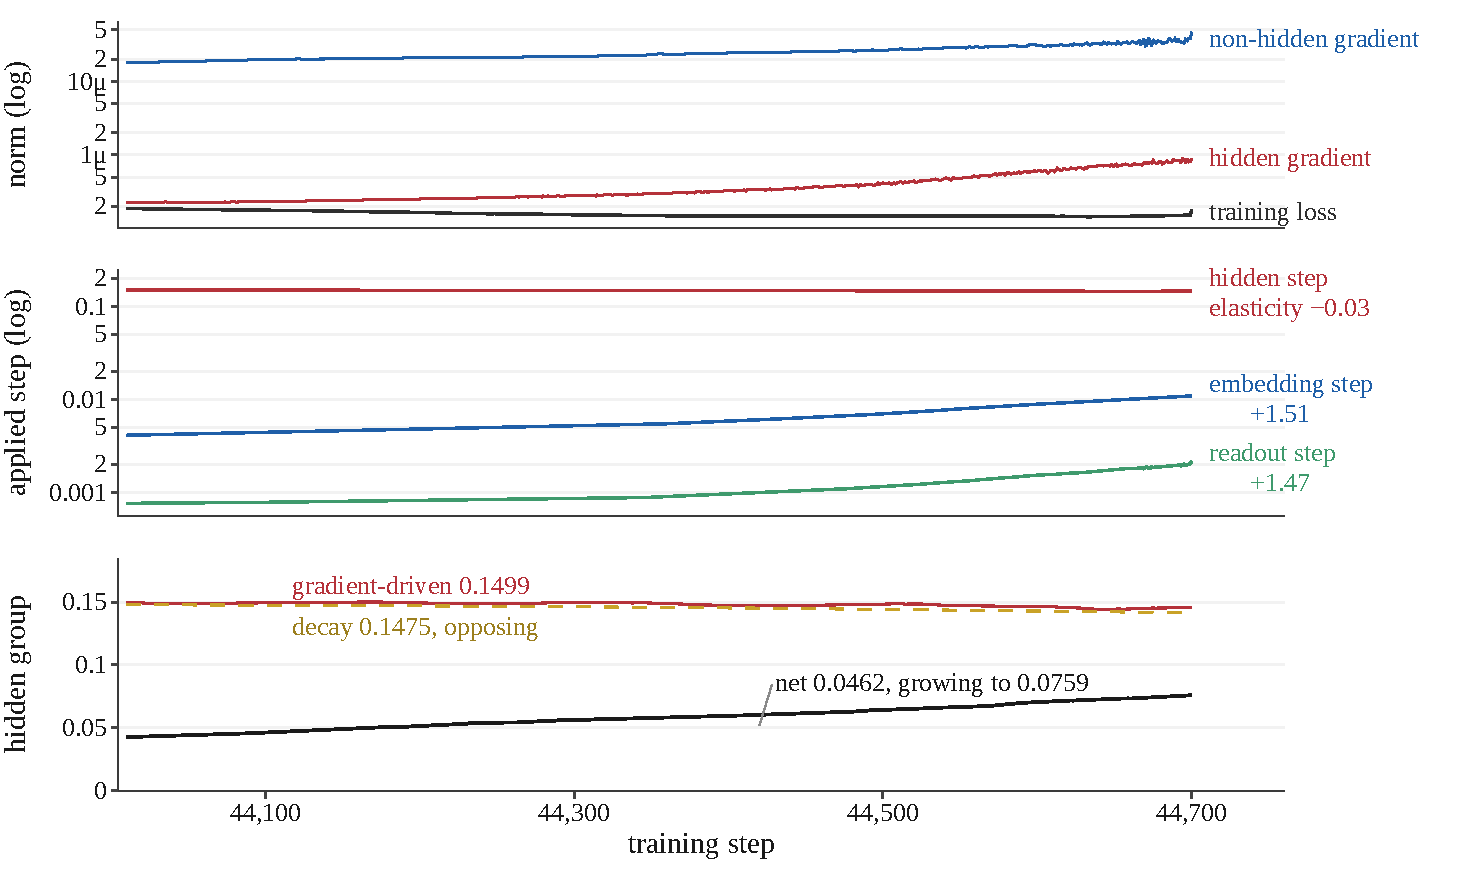
\includegraphics[width=\textwidth]{figure2_quiet.pdf}
\caption{Every-step measurements over $691$ updates before a collapse. \textbf{Top:} loss and gradient norms in the quiet window. \textbf{Middle:} gradient-driven applied steps and log--log slopes against the hidden gradient norm for Muon and the combined non-hidden norm for both AdamW groups. \textbf{Bottom:} hidden step and decay magnitudes differ by under $2\%$ at step $44{,}100$. Their vector sum is smaller and grows by $64\%$ from step $44{,}100$ to $44{,}700$ while the gradient-driven step changes little.}
\label{fig:quiet}
\end{figure}

\begin{table}[t]
\centering\small
\caption{Diagnostics through the quiet window and across the collapse. The training loss
and both gradient norms are numerically negligible until the failure. The Muon update column
is the orthogonalized step before weight decay, constant to within three percent; the net
displacement after decay is smaller and grows across the window, and is reported in the
text.}
\label{tab:quiet}
\begin{tabular}{lrrrr}
\toprule
Step & Train loss & Hidden grad.\ norm & Non-hidden grad.\ norm & Muon update norm \\
\midrule
$44{,}100$ & $1.77\times10^{-7}$ & $2.33\times10^{-7}$ & $1.95\times10^{-5}$ & $0.1498$ \\
$44{,}300$ & $1.55\times10^{-7}$ & $2.73\times10^{-7}$ & $2.20\times10^{-5}$ & $0.1494$ \\
$44{,}500$ & $1.50\times10^{-7}$ & $4.06\times10^{-7}$ & $2.67\times10^{-5}$ & $0.1481$ \\
$44{,}700$ & $1.53\times10^{-7}$ & $8.64\times10^{-7}$ & $3.52\times10^{-5}$ & $0.1455$ \\
\midrule
$44{,}710$ & $57.50$ & $25.26$ & $836.10$ & $0.1429$ \\
$44{,}720$ & $6.58$ & $5.09$ & $92.55$ & $0.1655$ \\
\bottomrule
\end{tabular}
\end{table}


Figure~\ref{fig:quiet} uses the every-step instrumented rerun, with a quiet window from $44{,}010$ through $44{,}700$ and failure at $44{,}702$. Table~\ref{tab:quiet} uses a separate ten-step spectral replay, whose first observed failure is at $44{,}710$. The following step/decay diagnostics use the instrumented rerun. On the hidden group the gradient-driven component is $0.1499$ at step $44{,}100$ against a decay component of $0.1475$, a ratio of $0.984$, leaving a net displacement of $0.0462$ that grows to $0.0759$ across the window while the orthogonalized step stays flat; over the window the hidden gradient norm grows by $3.92$ while its gradient-driven step changes by $0.97$, and the non-hidden gradient grows by $2.60$ while the embedding and readout steps grow by $2.65$ and $2.84$. The readout decay component has larger norm than its gradient-driven component on $14.9\%$ of quiet-window steps. In the ten-step spectral replay, the combined non-hidden gradient norm rises from $3.52\times10^{-5}$ to $836.10$; the orthogonalized Muon step over that interval is $0.1429$, lower than the $0.1455$ preceding it, and its maximum over the branch occurs after the event.

\section{Ablating the normalized-orthogonalization path}
\label{app:ablation}

\begin{table}[t]
\centering\small
\caption{Ablated runs that reach sustained generalization. Minimum is the lowest test
accuracy from the sustained-$95$ step to the last recorded evaluation. Terminal is the step
at which the loss becomes non-finite.}
\label{tab:nons}
\begin{tabular}{llrrrr}
\toprule
Learning rate & Backend & Precision & Grokked & Minimum & Terminal \\
\midrule
$0.3$ & MPS & \texttt{float32} & $3{,}100$ & $97.28\%$ & $23{,}514$ \\
$0.3$ & CPU & \texttt{float32} & $3{,}100$ & $97.52\%$ & $24{,}485$ \\
$0.3$ & CPU & \texttt{float64} & $3{,}100$ & $97.06\%$ & $22{,}889$ \\
$1.0$ & MPS & \texttt{float32} & $6{,}800$ & $97.11\%$ & $23{,}800$ \\
$1.0$ & CPU & \texttt{float64} & $7{,}700$ & $95.96\%$ & $29{,}831$ \\
$1.0$ & CPU & \texttt{float32} & $6{,}500$ & $95.60\%$ & $38{,}955$ \\
\bottomrule
\end{tabular}
\end{table}


The ablation removes Frobenius normalization and the Newton--Schulz iteration together, retaining momentum, shape scaling, and weight decay. In the tested sweep, learning requires a rate of $0.3$ or $1.0$. Six ablated runs generalize, with no recorded post-grokking evaluation below $95\%$ (Table~\ref{tab:nons}). All six were observed to terminate with non-finite loss, in float32 and float64, at steps $22{,}889$--$38{,}955$. The matched Muon comparator records thirteen sub-threshold evaluations through step $22{,}800$. Over its full $100{,}000$ steps, its minimum and final accuracies are $29.49\%$ and $96.48\%$. At the analyzed checkpoints, ablation reduces dispersion from $326.09$ effective conjugate pairs to $4.11$, while the task-aligned family retains $100\%$ sufficiency (Appendix~\ref{app:dispersion}).

\section{Prevention details}
\label{app:prevention}

\begin{table}[t]
\centering\small
\caption{Stable Muon across five runs covering four settings; the main condition appears
twice, under a fixed freeze step and under the automatic trigger. The minimum is the lowest
test accuracy at
any evaluation from the sustained-$95$ step onward, and in every run it is the value at
that step itself.}
\label{tab:stable}
\begin{tabular}{lrrrrr}
\toprule
Run & Grokked & \shortstack{First frozen\\eval.} & Post-grokking steps & Minimum & Evals $<95\%$ \\
\midrule
Main condition & $5{,}900$ & $8{,}100$ & $94{,}100$ & $95.34\%$ & $0$ \\
Selected Stable Muon & $5{,}400$ & $7{,}500$ & $94{,}600$ & $95.74\%$ & $0$ \\
$p = 97$ & $6{,}300$ & $8{,}400$ & $93{,}700$ & $95.05\%$ & $0$ \\
Training fraction $20\%$ & $14{,}500$ & $16{,}600$ & $85{,}500$ & $95.16\%$ & $0$ \\
Width $64$ & $16{,}500$ & $18{,}600$ & $83{,}500$ & $95.67\%$ & $0$ \\
\midrule
Total & & & $451{,}400$ & & $0$ \\
\bottomrule
\end{tabular}
\end{table}


In four of the five runs the freeze is triggered automatically, $2{,}000$ steps after the first evaluation of a five-evaluation streak at or above $95\%$; the main-condition run uses a fixed step. The first logged frozen evaluation lands $2{,}100$ to $2{,}200$ steps after sustained generalization; the actual freezes occur $100$ steps earlier. Within a depth-2 run the median step costs $57.87$\,ms before the freeze and $54.72$ after; at depth 4, $111.39$ and $107.75$; pre-freeze rates match ordinary Muon's. Holding only the unembedding constant from the same step leaves the run unstable, minimum $83.13\%$ and eighteen of $936$ evaluations below $95\%$; freezing the embeddings and unembedding together at the same step produces none.

\section{Fourier decomposition and intervention suite}
\label{app:fourier}

\begin{table}[t]
\centering\small
\caption{The six mode families. The families are pairwise disjoint and exhaust the
$p \times p$ grid, so any statement about one family and its complement is an exact
accounting of the whole representation.}
\label{tab:families}
\begin{tabular}{lll}
\toprule
Family & Modes & Count at $p = 113$ \\
\midrule
Addition & $(k, k)$, $k \neq 0$ & $112$ \\
Subtraction & $(k, -k)$, $k \neq 0$ & $112$ \\
$a$-only & $(k, 0)$, $k \neq 0$ & $112$ \\
$b$-only & $(0, l)$, $l \neq 0$ & $112$ \\
Constant & $(0, 0)$ & $1$ \\
Generic interaction & all remaining $(k, l)$ & $12{,}320$ \\
\midrule
Total & & $12{,}769$ \\
\bottomrule
\end{tabular}
\end{table}

\begin{table}[t]
\centering\small
\caption{Interventions applied to a cached state. Each is designed to hold one property of
the representation fixed while destroying another, so that a drop in accuracy attributes
to the property destroyed.}
\label{tab:interventions}
\begin{tabular}{lll}
\toprule
Intervention & Preserved & Destroyed \\
\midrule
Family sufficiency & Modes in one family & All other families \\
Family ablation & All other families & Modes in one family \\
Equal-power relocation & Total power, family membership & Which frequencies carry it \\
Random native subset & Family membership, power scale & Which of the used frequencies survive \\
Pair-global phase scramble & Support and power exactly & Relative phase across pairs \\
Channelwise phase scramble & Support and power exactly & Relative phase across channels \\
Cross-readout substitution & Both representations intact & Pairing of state with its own readout \\
\bottomrule
\end{tabular}
\end{table}

\begin{table}[t]
\centering\small
\caption{Family interventions at forty-three solved checkpoints, spanning five seeds and the
Muon, Stable Muon, and AdamW regimes. Sufficiency retains only the named family; ablation
removes it and retains the rest. The chance rate is $0.88\%$.}
\label{tab:families-result}
\begin{tabular}{lrrrr}
\toprule
Family & Sufficiency & Range & Ablation & Range \\
\midrule
Addition & $100.00\%$ & $[100.00,\,100.00]$ & $1.71\%$ & $[0.67,\,4.24]$ \\
Subtraction & $0.88\%$ & $[0.88,\,0.88]$ & $99.61\%$ & $[95.79,\,100.00]$ \\
$a$-only & $0.88\%$ & $[0.88,\,0.88]$ & $99.85\%$ & $[97.76,\,100.00]$ \\
$b$-only & $0.88\%$ & $[0.88,\,0.88]$ & $99.85\%$ & $[97.72,\,100.00]$ \\
Constant & $0.88\%$ & $[0.88,\,0.88]$ & & \\
Generic interaction & $3.28\%$ & $[0.78,\,14.21]$ & $99.99\%$ & $[99.78,\,100.00]$ \\
\bottomrule
\end{tabular}
\end{table}


For a chosen point in the forward pass the model runs on all $p^2$ operand pairs, the states form a tensor $X\in\mathbb{R}^{p\times p\times d}$, and an orthonormal two-dimensional DFT over the operand axes gives $\widehat{X}[k,l,:]$ with power $\lVert\widehat{X}[k,l,:]\rVert^2$. Because $X$ is real, modes occur in conjugate pairs and every filter retains or removes both members together; transforms run in single precision on CPU. The families of Table~\ref{tab:families} are pairwise disjoint and exhaust the grid, and addition and subtraction are disjoint because $p$ is odd. Power fractions are normalized against non-constant power; every non-constant-family sufficiency filter also retains the constant mode, which becomes a fixed logit offset under the bias-free unembedding. Ablation removes only the selected non-constant modes, retaining this offset. The two masks are complementary on the non-constant spectrum and share the constant mode. In the margin decomposition and $\alpha$ sweep, the task-aligned component excludes the constant mode, which belongs to the remainder. Solved-checkpoint selection and intervention accuracies use the full operand grid; training trajectories explicitly labeled test accuracy use the held-out split.

Table~\ref{tab:families-result} applies sufficiency and ablation to each family at forty-three solved checkpoints spanning five seeds and the Muon, Stable Muon, and AdamW regimes. Equal-power relocation ranges $0.88\%$ to $15.04\%$ over $430$ replicates. Among the tested descending-power prefixes, the smallest reaching $95\%$ contains two to four conjugate pairs at AdamW checkpoints (median $3$), against three to seventeen at Muon (median $12.5$) and eight to nineteen at Stable Muon (median $11$). Along the AdamW trajectory of \S\ref{sec:outvoted}, the five strongest pairs give $4.91\%$ at step $3{,}000$, $19.48\%$ at $20{,}000$, $70.73\%$ at $30{,}000$, and $100\%$ at $37{,}000$, while the family's share rises from $1.05\%$ through $1.66\%$ and $11.08\%$ to $70.62\%$, reaching $90.51\%$ by step $100{,}000$; test accuracy over those steps is $0.30\%$, $0.29\%$, $2.08\%$, and $100\%$.

The full-family accuracies above include the orbit average in Eq.~\ref{eq:orbit-average}. Prefix filtering and phase or frequency perturbations measure additional spectral structure, but their interpretation as evidence of a learned algorithm requires controls against memorization. Appendix~\ref{app:fourier-control} supplies that comparison.

\section{Spectral dispersion}
\label{app:dispersion}

\begin{figure}[t]
\centering
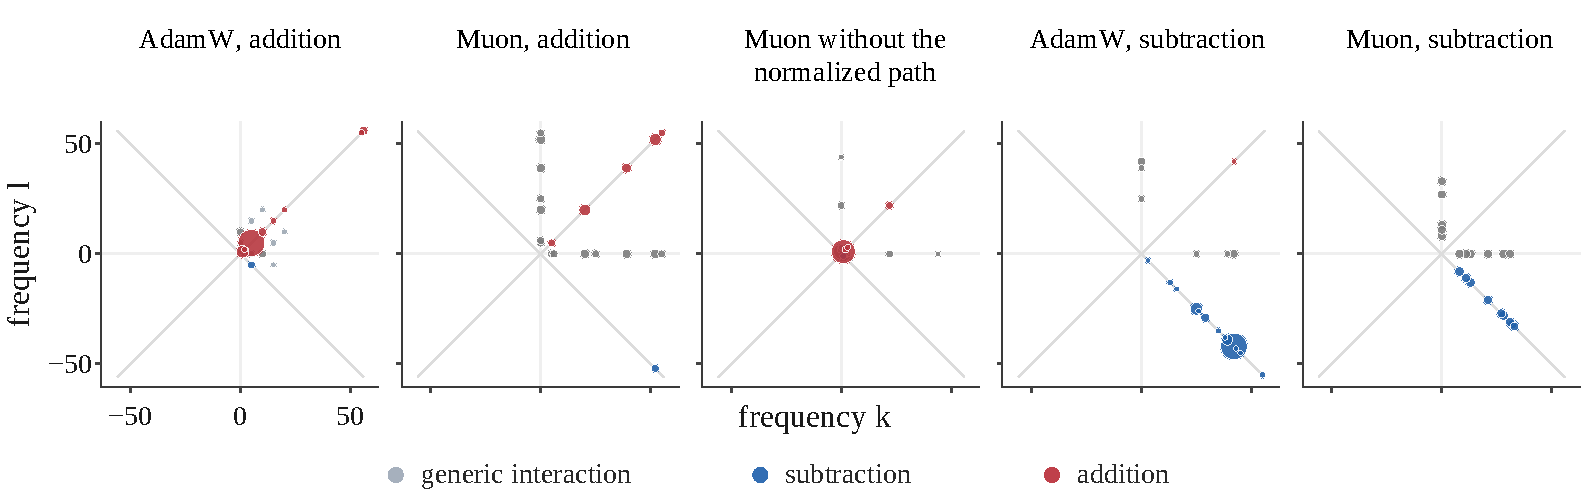
\includegraphics[width=\textwidth]{figure4_grid.pdf}
\caption{The twenty highest-power conjugate pairs of the final residual at converged checkpoints, on the mode grid, sized by share of non-constant power; grey lines mark $l=k$ and $l=-k$. AdamW places $80.1\%$ of non-constant power on a single pair of the family the task selects; Muon's strongest pair carries $7.9\%$, with the rest spread across the family and beyond it; ablating the normalized path returns the strongest pair to $58.9\%$. Between the addition and subtraction panels the occupied line moves from one diagonal to the other.}
\label{fig:grid}
\end{figure}

\begin{table}[t]
\centering\small
\caption{Spectral dispersion at solved checkpoints of the matched depth-$1$ runs. Effective
pairs is $\exp(-\sum_i q_i\log q_i)$, with normalized pair powers $q_i$, over all $6{,}384$ non-constant conjugate pairs,
reported as a mean with range. Family power is the task-aligned family's share of
non-constant power, meaning $(k,k)$ for addition and $(k,-k)$ for subtraction, and top-five
power is the share carried by the five strongest pairs of the spectrum. The final row ablates the normalization and orthogonalization together.}
\label{tab:sparsity}
\begin{tabular}{llrrr}
\toprule
Operation & Optimizer & Effective pairs & Family power & Top-five power \\
\midrule
Addition & AdamW & $4.95$ \ \ $[3.68,\,10.20]$ & $91.0\%$ & $93.7\%$ \\
Addition & Muon & $326.09$ \ \ $[96.91,\,578.90]$ & $28.0\%$ & $13.1\%$ \\
\midrule
Subtraction & AdamW & $2.54$ \ \ $[2.45,\,2.72]$ & $95.4\%$ & $96.5\%$ \\
Subtraction & Muon & $211.46$ \ \ $[33.25,\,377.24]$ & $27.7\%$ & $16.0\%$ \\
\midrule
Addition & Muon, path ablated & $4.11$ \ \ $[2.04,\,6.05]$ & $66.5\%$ & $94.0\%$ \\
\bottomrule
\end{tabular}
\end{table}


Table~\ref{tab:sparsity} reports the entropy effective count $\exp(-\sum_i q_i\log q_i)$ over all $6{,}384$ non-constant conjugate pairs and the task-aligned family's power share on matched depth-1 runs. Here $q_i$ denotes normalized pair power. Across the five-seed study AdamW occupies $4.40$ effective pairs on average over thirty solved checkpoints, Muon $385.85$ over twenty-five, and Stable Muon $343.96$ over thirty-six: freezing the interface leaves the dispersion where Muon put it and removes the instability anyway. Within each family's $(p-1)/2$ pairs, the generality analysis instead uses the inverse participation ratio $1/\sum_i q_i^2$, with $q_i$ renormalized within the family: $1.99$--$2.59$ for solved AdamW variants and $21.33$--$55.34$ for Muon. On the uniform operand grid, a predictor using only the opposite family and a constant offset has accuracy exactly $1/p$, since sum and difference are independent for odd $p$. Across solved matched checkpoints, AdamW places $0.0$--$7.8\%$ of non-constant power there and Muon $2.5$--$17.7\%$.

\section{The matched branch through failure, recovery, and masking}
\label{app:branchtraj}

\begin{table}[t]
\centering\small
\caption{The addition family along matched branches. Pairs counts how many of the twenty
highest-power conjugate pairs at the final residual belong to the family; share is the
family's fraction of non-constant power; addition-only is accuracy when the representation
is filtered to the family.}
\label{tab:coordinates}
\begin{tabular}{lrrrrr}
\toprule
Step & Branch & Pairs & Share & Addition-only & Full \\
\midrule
$126{,}200$ & control & $11$ & $83.95\%$ & $100.00\%$ & $94.07\%$ \\
$126{,}200$ & freeze & $11$ & $83.95\%$ & $100.00\%$ & $94.07\%$ \\
\midrule
$160{,}000$ & control & $1$ & $11.88\%$ & $2.65\%$ & $3.29\%$ \\
$160{,}000$ & freeze & $12$ & $89.33\%$ & $100.00\%$ & $98.97\%$ \\
$180{,}000$ & control & $0$ & $0.32\%$ & $0.88\%$ & $0.97\%$ \\
$180{,}000$ & freeze & $12$ & $88.32\%$ & $100.00\%$ & $97.95\%$ \\
$230{,}000$ & control & $4$ & $67.69\%$ & $100.00\%$ & $98.41\%$ \\
$230{,}000$ & freeze & $12$ & $90.78\%$ & $100.00\%$ & $99.47\%$ \\
$300{,}000$ & control & $3$ & $20.38\%$ & $100.00\%$ & $45.85\%$ \\
$300{,}000$ & freeze & $12$ & $90.69\%$ & $100.00\%$ & $98.89\%$ \\
\bottomrule
\end{tabular}
\end{table}


Table~\ref{tab:coordinates} follows the family's top-twenty membership, power share, isolated accuracy, and full-model accuracy along the depth-4 matched pair of \S\ref{sec:outvoted} from a bit-identical state. Over $174{,}000$ steps, the frozen branch retains high filtered accuracy and substantial family power; the control loses all three at filtered-pathway failure through its current readout, recovers all three, and loses the share again at projection masking while the isolated family still gives $100\%$. The $\alpha$-sweep crossing at $\alpha=2.55$ occurs at a share of $0.6247$, below the frozen branch's native $0.9069$. Replaying a depth-1 collapse and recovery at ten-step resolution: full accuracy returns to $99.90\%$ within $300$ steps while the addition-family power cosine to the pre-collapse state reaches only $0.55$; the pre-collapse representation holds between $4.2\%$ and $5.7\%$ under the recovered readout throughout, while the recovered representation reads at $90.73\%$ under the pre-collapse readout. The matched branches' five strongest modes are identical at the branch point and share at most one pair at sampled steps $160{,}000$ through $230{,}000$. Patching the addition component of the frozen branch's final MLP write into the control under the frozen readout gives $99.99\%$; under the control's own readout, $5.05\%$; patching its full final MLP write gives $97.61\%$ and $4.46\%$ under the two readouts; patching only the non-addition component of that MLP write into the control gives $36.79\%$, below the control's unmodified $45.85\%$.

\section{Depth}
\label{app:depth}

\begin{table}[t]
\centering\small
\caption{Time to sustained generalization, in optimizer steps and in elapsed seconds on a
single device. Per-step cost is the median over evaluation intervals. The AdamW baseline at
depth $4$ is right-censored at the step budget.}
\label{tab:wallclock}
\begin{tabular}{llrrrr}
\toprule
Depth & Optimizer & ms/step & Steps to grok & Seconds to grok & Advantage \\
\midrule
\multirow{2}{*}{$2$} & AdamW & $33.06$ & $5{,}100$ & $170$ & \\
 & Muon & $57.81$ & $2{,}300$ & $133$ & $2.22\times$ steps, $1.28\times$ time \\
\midrule
\multirow{2}{*}{$4$} & AdamW & $61.68$ & $>300{,}000$ & $>19{,}768$ & \\
 & Muon & $110.87$ & $52{,}600$ & $5{,}856$ & $>5.70\times$ steps, $>3.37\times$ time \\
\bottomrule
\end{tabular}
\end{table}

\begin{table}[t]
\centering\small
\caption{Stage-level interventions at depth $4$, step $53{,}000$, baseline $99.30\%$.
Relocation transports the addition family onto other diagonal frequencies at matched power;
phase scrambling randomizes the phase of each conjugate pair. The two stochastic columns
show the reported realization (replicate $4$ of five); zeroing is deterministic.}
\label{tab:stagewise}
\begin{tabular}{llrrr}
\toprule
Stage & Kind & Relocation & Phase & Zeroed \\
\midrule
Block 1 attention write & write & $99.30\%$ & $99.30\%$ & $86.31\%$ \\
Block 2 attention write & write & $99.33\%$ & $99.29\%$ & $0.94\%$ \\
Block 3 attention write & write & $99.29\%$ & $99.30\%$ & $0.44\%$ \\
\midrule
Block 3 MLP activation & activation & $1.66\%$ & $0.00\%$ & $1.19\%$ \\
Block 3 MLP write & write & $0.95\%$ & $0.00\%$ & $1.19\%$ \\
Block 4 attention write & write & $3.58\%$ & $0.00\%$ & $58.44\%$ \\
\bottomrule
\end{tabular}
\end{table}

\begin{table}[t]
\centering\small
\caption{Direct-readout accuracy by post-block residual, decoding with the final unembedding and
skipping the remaining blocks. Values are ranges over the same $41$ checkpoints used in
Section~\ref{sec:depth}, each with native full-grid accuracy of at least $95\%$. Both columns
report percentages to two decimal places.}
\label{tab:depthreadout}
\begin{tabular}{llrr}
\toprule
Depth & Regime & Earlier blocks & Final block \\
\midrule
$2$ & AdamW & $0.72$--$0.88\%$ & $99.99$--$100.00\%$ \\
$2$ & Muon & $0.85$--$5.09\%$ & $95.83$--$99.95\%$ \\
$2$ & Stable Muon & $1.28$--$5.23\%$ & $96.37$--$99.40\%$ \\
$4$ & Muon & $0.78$--$17.97\%$ & $95.07$--$99.30\%$ \\
$4$ & Stable Muon & $0.69$--$17.58\%$ & $95.25$--$98.71\%$ \\
\bottomrule
\end{tabular}
\end{table}

\begin{figure}[t]
\centering

\includegraphics[width=\textwidth]{figure6_depth.pdf}
\caption{A depth-$4$ Muon checkpoint. Left: accuracy after intervening on each stage in
forward order. Relocating the task-aligned family onto other frequencies and scrambling its
phase leave the model above $99\%$ at every stage through the block-$3$ attention write and
destroy it at the block-$3$ MLP activation; the two coincide before the cliff. Zeroing a stage destroys
accuracy everywhere, so earlier stages are computationally necessary while carrying no
frequency- and phase-specific code. Right: decoding a post-block residual directly with the
unembedding, for the state itself and for its task-aligned part alone. Neither is legible
before the final block, and the task-aligned part is the more legible of the two wherever
both are partial.}
\label{fig:depth}
\end{figure}


Muon reaches sustained generalization in $2{,}300$ steps at depth 2 against $5{,}100$, and in $52{,}600$ at depth 4 where AdamW peaks at $96.69\%$ and never sustains the threshold within $300{,}000$ steps. Table~\ref{tab:wallclock} compares steps and elapsed time; a Muon step costs $1.75$--$1.80\times$ an AdamW step. At the depth-4 checkpoint in Table~\ref{tab:stagewise}, zeroing the block-2 and block-3 attention writes leaves $0.94\%$ and $0.44\%$ accuracy. Frequency relocation and phase scrambling at these writes preserve near-baseline accuracy. Both perturbations cause a large drop at the block-3 MLP activation. Figure~\ref{fig:depth} and Table~\ref{tab:stagewise} show the reported perturbation realization. Later-stage outcomes vary across the five perturbations, so near-chance accuracy in this realization does not establish uniform sensitivity across perturbations.

Across eleven solved checkpoints, the first stage where mean pair-phase scrambling costs more than half the baseline accuracy is an MLP activation in ten and an MLP write in one. This criterion averages five perturbations per stage. Direct decoding reaches $95\%$ only at the final block across all $41$ checkpoints selected by full-grid accuracy, never exceeding $17.97\%$ earlier (Table~\ref{tab:depthreadout}). Within the eleven-checkpoint stage-intervention subset, among seventeen residual states with direct-readout accuracy between $2\%$ and $95\%$, family filtering improves sixteen, with a mean increase of $4.88$ percentage points across all seventeen. Across eighteen depth-4 checkpoints after the shared state, between-branch power cosine stays above $0.98$ in the first block; in the fourth it lies between $0.03$ and $0.44$ at fifteen checkpoints. The exact-state branch at step $126{,}200$ raises mean post-branch accuracy from $48.07\%$ to $97.50\%$, final accuracy from $36.88\%$ to $98.87\%$, and cuts evaluations below $90\%$ from $1{,}353$ to $66$.
